% INTRO
% intro sobre qué queremos (programa que soluciona problemas por nosotros)
% qué toma de input (autómatas, modelo de la realidad, en general son varios)
% detalles de los autómatas (estado inicial, marcados, etc) con ejemplo de avión
% la composición explota, los algor clásicos rompen acá (i.e. decir que existe algor monolítico)
% idea general: componer mientras exploras y terminar al tener conclusión (con suerte antes de ver todo)
% [buscar] ejemplo simple para explicar composición (mostrar planta completa)
%-------------------------------------------------------
\begin{frame}{Objetivo}
    \begin{block}{}
    ``The good thing about computers is that they do what you tell them to do. The bad news is that they do what you tell them to do.''\hfill – Ted Nelson 
    \end{block}
    
    \pause
    ¿Es posible hacer que una computadora se diga a sí misma qué hacer?
    
    \pause
    \begin{block}{Síntesis Automática de Controladores}
     Se le brinda a un programa las reglas y objetivos a cumplir, éste sintetiza una estrategia para ganar (si existe) conocida con el nombre de controlador.
    \end{block}

\end{frame}
%-------------------------------------------------------
\begin{frame}{Control de Eventos Discretos}
    \begin{itemize}
     \item Es una de las áreas que estudia problemas de síntesis.
     \item El problema es modelado usando autómatas finitos (o máquinas de estados finitos).
     \pause
     \item Estos autómatas modelan la parte que nos interesa de la realidad.
     \item Se suele partir el modelo en pequeñas partes, más simples de abstraer, y luego se componen para formar el objeto de interés.
    \end{itemize}
\end{frame}
%-------------------------------------------------------
\begin{frame}{Autómatas} 
    \begin{figure}
     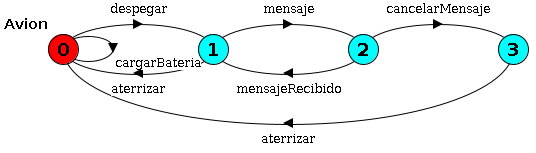
\includegraphics[width=\textwidth]{figures/avion.png}
    \end{figure}

    \begin{itemize}
     \item Estados finitos, en este caso del 0 al 3 (4 estados).
     \item Estado inicial, en los ejemplos siempre será el 0.
     \item Acciones o eventos, en el ejemplo: despegar, aterrizar, cargarBateria, mensaje, mensajeRecibido, cancelarMensaje.
    \end{itemize}
    
\end{frame}
%-------------------------------------------------------
\begin{frame}{Componentes}
    \begin{figure}
     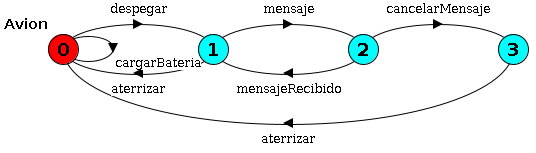
\includegraphics[width=\textwidth]{figures/avion.png}
     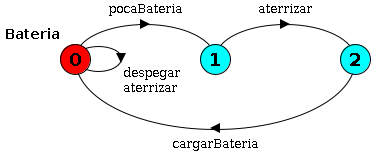
\includegraphics[width=0.6\textwidth]{figures/bateria.png}
    \end{figure}
\end{frame}
%-------------------------------------------------------
\begin{frame}{Composición}
    \begin{figure}
     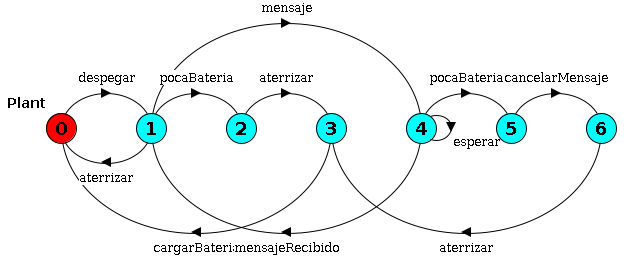
\includegraphics[width=\textwidth]{figures/planta.png}
    \end{figure}
    En nuestro caso el autómata \textit{Batería} contiene la información de cómo actuar (qué acciones se pueden hacer) en caso de tener poca batería.\\ 
    Al componer con el autómata \textit{Avión} se restringen las acciones pero también hay un aumento de estados; ya que no es lo mismo estar en el aire con poca batería o completa.
%     explicar por arriba cómo se compone o cuál es la idea (la planta refleja el comportamiento del todo) (reglas para sincronización entre las partes) NO QUEDARA MUY TECNICO ESTO?
\end{frame}
%-------------------------------------------------------
\begin{frame}{Explosión de estados}
    La composición muchas veces explota en tamaño y termina siendo prohibitiva para algoritmos monolíticos (los que analizan la planta completa). Así queda el muy simple ejemplo anterior si la batería tiene un contador de carga:
    \begin{figure}
    	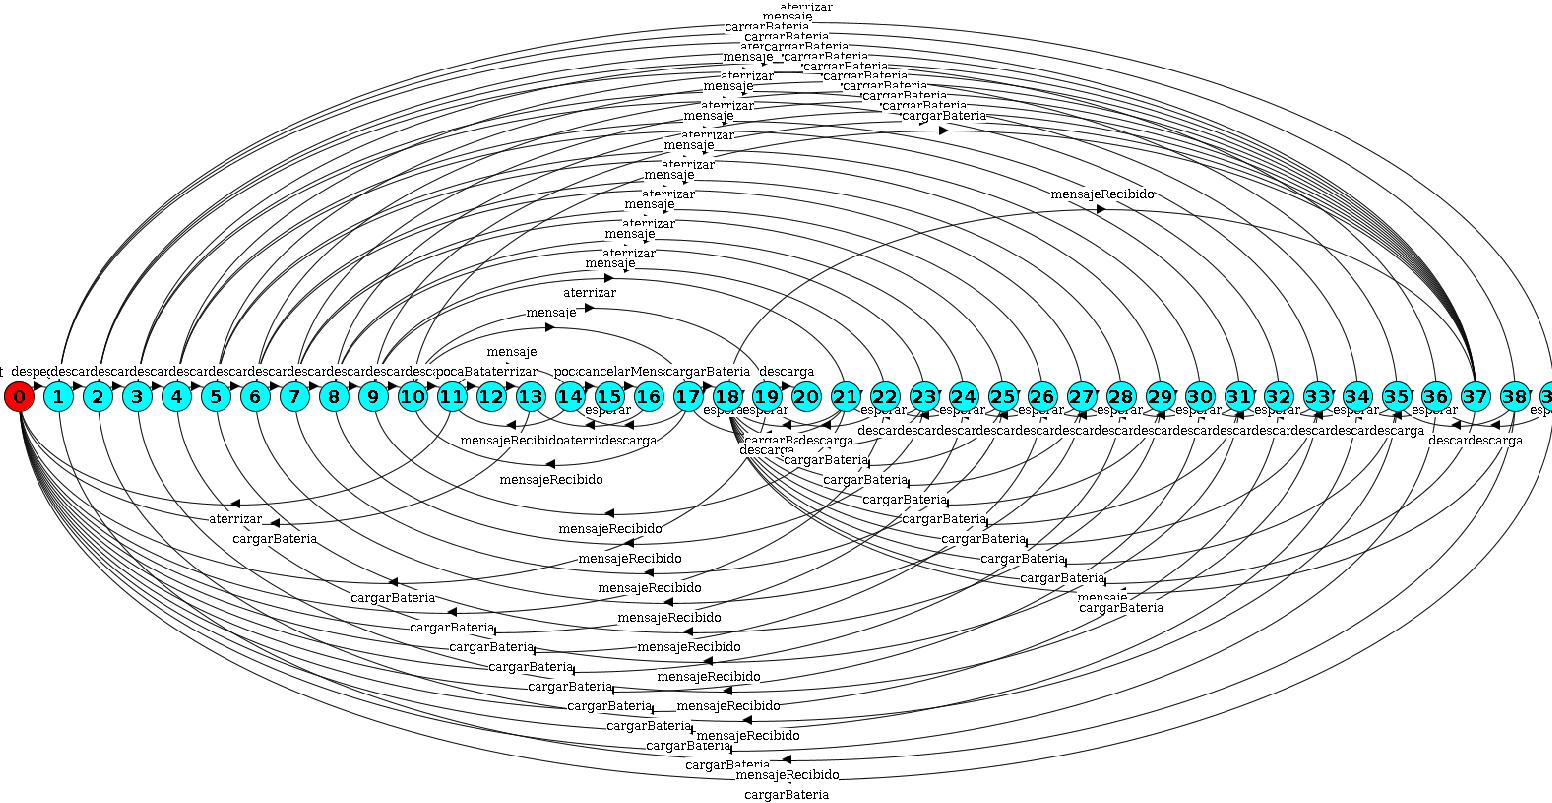
\includegraphics[width=\textwidth]{figures/big-plant.png}
    \end{figure}
\end{frame}
%-------------------------------------------------------
\begin{frame}{Idea general de este trabajo}
    Partiendo de las ideas presentadas en la tesis doctoral de Daniel Ciolek, queremos componer mientras se explora y terminar al tener una conclusión (con suerte antes de ver toda la composición).
    \bigskip
    
    La tesis doctoral incluye un algoritmo de exploración pero presenta algunos errores a la hora de clasificar los estados. Nuestro trabajo se centró en \textbf{diseñar un nuevo algoritmo} que solucione esos errores, y dar una \textbf{demostración} formal al respecto.
    
\end{frame}
%-------------------------------------------------------
